\chapter{Monitorowanie procesu gojenia ścięgna Achillesa}
\section{Ścięgno Achillesa}
Ścięgno Achillesa, nazywane również ścięgnem piętowym, jest największym i zarazem wytrzymującym największe obciążenia ścięgnem występującym w ciele ludzkim. Stanowi wspólne zakończenie mięśnia trójgłowego łydki, w którego skład wchodzą dwie głowy mięśnia brzuchatego i mięsień płaszczkowaty. Całość struktury zlokalizowana jest w tylnym, powierzchownym przedziale łydki, co zobrazowano \linebreak na Rysunku \ref{muscle_structure}.  
\begin{figure}[h!]
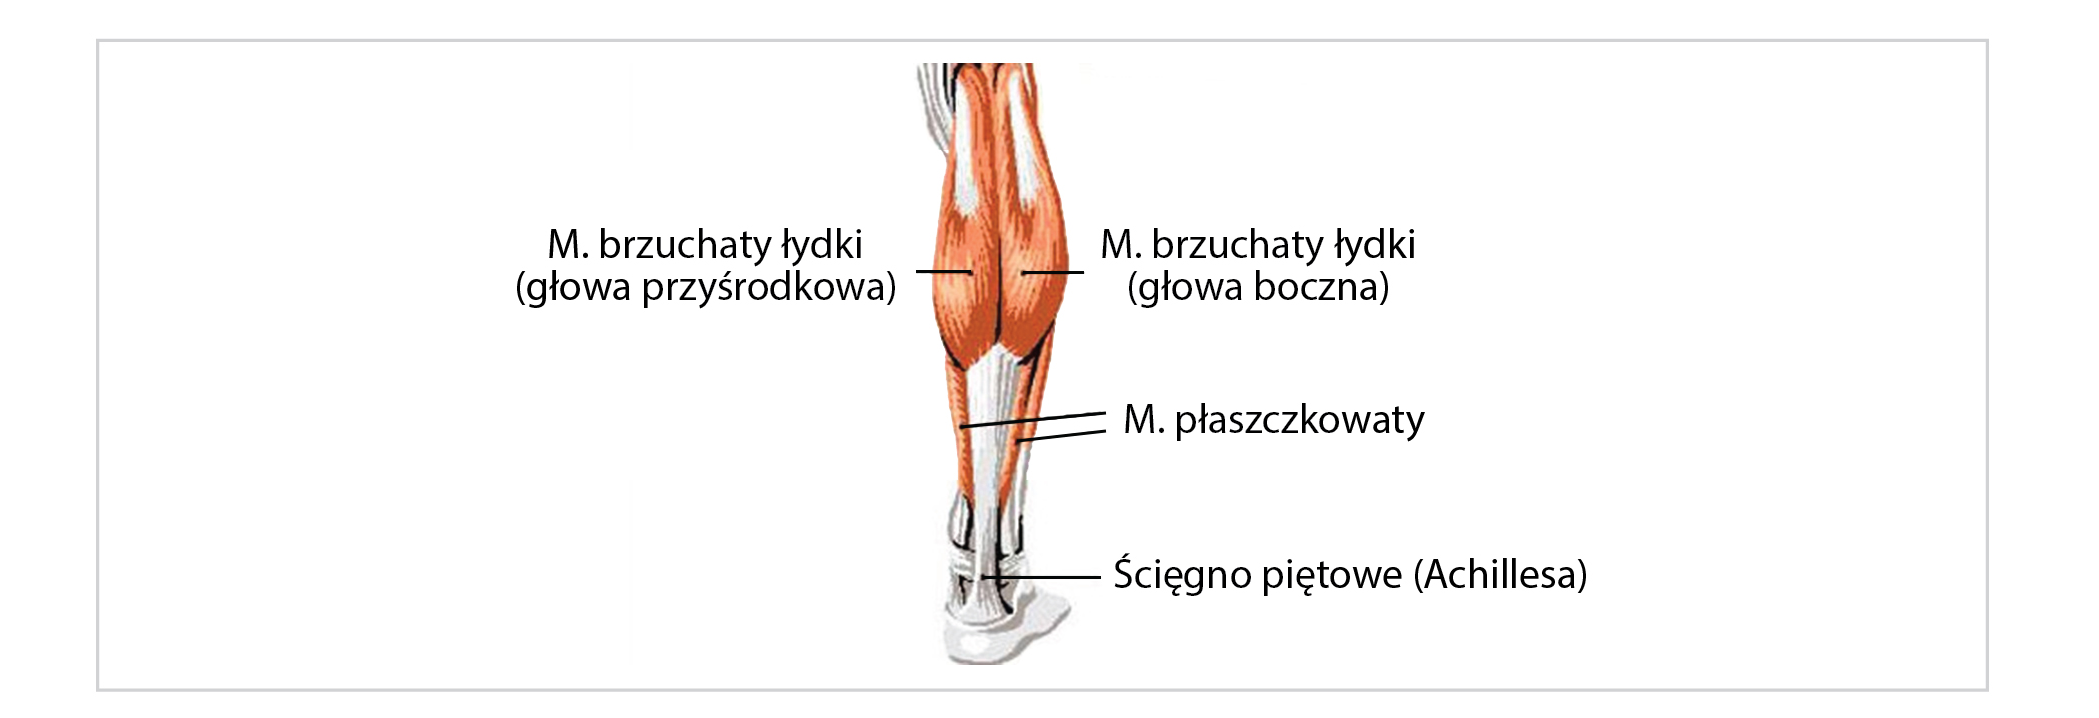
\includegraphics[width=1\textwidth]{figures/muscleStructure.png}
\caption{Lokalizacja mięśnia trójgłowego łydki wraz ze ścięgnem Achillesa (na podst. \cite{Doral2010}).}
\label{muscle_structure}
\end{figure}
\newpage
Procesy patofizjologiczne zachodzące po urazie ścięgna są ściśle związane z jego anatomią, biomechaniką, typem urazu i czynnikami jemu sprzyjającymi. Wszystkie te aspekty mają wpływ na możliwość monitorowania procesów gojenia się ścięgna \linebreak i jego wspomagania. Dlatego zostaną szczegółowo omówione w kolejnych punktach. 

\subsection{Anatomia}
\label{anatomia}

Z obu głów (brzuśców) mięśnia brzuchatego łydki wyrasta jedno szerokie, płaskie pasmo, które jest początkiem części brzuchatej ścięgna Achillesa. Następnie ścięgno to łączy się z włóknami pochodzącymi od mięśnia płaszczkowatego, które układają się stycznie do wcześniej powstałej struktury. Podążając w dół łydki, kształt ścięgna Achillesa ulega stopniowemu zwężeniu i zaokrągleniu, aż do punktu o minimalnej szerokości (około 4 cm nad przyczepem dolnym -- za \cite{Doral2010}). W rejonie samego przyczepu, znajdującego się na guzie piętowym, ścięgno ponownie jest płaskie i szerokie.

Średnia długość ścięgna Achillesa to 15 cm (zakres to: 11 -- 26 cm). Średnia szerokość w rejonie początku wynosi 6,8 cm (4,5 -- 8,6 cm), w rejonie zwężenia \linebreak to 1,8 cm (1,2 -- 2,6 cm), a w miejscu przyczepu dolnego 3,4 cm (2,0 -- 4,8 cm) \cite{Doral2010, KoivunenNiemel1995}.

Ścięgno jest zbudowane z tkanki łącznej, a dokładniej mówiąc z tkanki łącznej właściwej zbitej. Składa się w przeważającej części z \textit{istoty międzykomórkowej} (nazywanej też \textit{macierzą międzykomórkową}) zbudowanej z istoty podstawowej (ang. \textit{ground substance}) oraz włókien. Dopełnienie struktury stanowią komórki takie jak fibroblasty, komórki tuczne, komórki plazmatyczne, histiocyty i komórki napływowe. 

Istota podstawowa jest rodzajem żelu wiążącym duże ilości wody, włókien i komórek. Pełni ona rolę otoczki zapewniając możliwość transportu wody i substancji odżywczych do wnętrza struktury \cite{Sharma2006}, gdzie znajdują się komórki poukładane \linebreak w wąskie pasy leżące pomiędzy włóknami \cite{Maffulli2005}. Wśród włókien można wyróżnić trzy rodzaje: kolagenowe, siateczkowe i sprężyste.

Włókna kolagenowe i siateczkowe są zbudowane z fibrylarnego białka -- kolagenu, najczęściej występującego białka w organizmie człowieka, stanowiącego około 25\% wszystkich białek. Makrocząsteczki kolagenu składają się ze zwiniętych łańcuchów polipeptydowych tworzących helisy. Dotychczas zidentyfikowano 20 typów kolagenu różniących się od siebie szczegółową budową helisy. Kolagen typu I stanowi około 90\% masy wszystkich typów włókien i jest podstawowym budulcem włókien kolagenowych tworzących zazwyczaj wiązki o grubości 50--100 $\mu$$m$. Włókna siateczkowe zbudowane są natomiast w przeważającym stopniu z kolagenu typu III. Pozostałe typy kolagenu występują w znacząco mniejszym stopniu tworząc włókienka kolagenowe i siateczkowe o różnej grubości -- od 10 do 300 nm (por. \cite{sawicki2008histologia}).

Włókna sprężyste występują w postaci sieci i mają średnicę 0,2--10 $\mu$$m$. Zbudowane są z \textit{elastyny}, rozciągliwego i sprężystego białka. Dzięki temu, włókna te pod wpływem działania siły zewnętrznej mogą zwiększać swoją długość nawet o 50\% (za. \cite{sawicki2008histologia}). 

W zdrowym ścięgnie Achillesa widoczne są ściśle upakowane włókna sprężyste \linebreak i kolagenowe. Włókna kolagenowe stanowią 70\% masy suchego ścięgna i charakteryzują się hierarchiczną strukturą zobrazowaną na Rys. \ref{Achilles-histology}.  
\begin{figure}[h!]
	\centering
	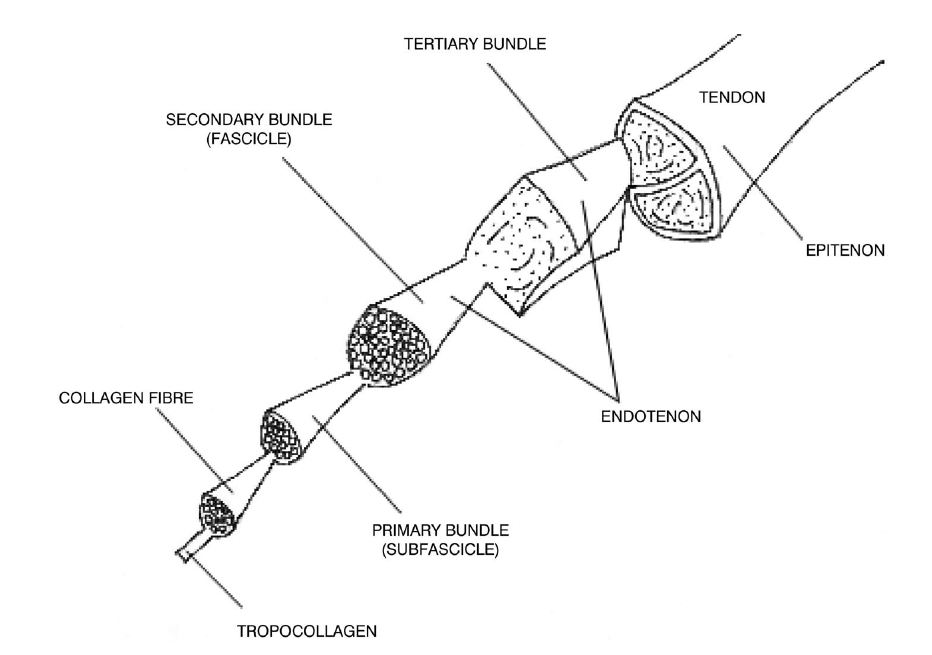
\includegraphics[width=1\textwidth]{figures/Achilles_hist.png}
	\caption{Schemat hierarchicznej budowy ścięgna Achillesa (na podst. \cite{Sharma2006}).}
	\label{Achilles-histology}
\end{figure}

Wyróżnić można: włókna, wiązki pierwszo, drugo i trzeciorzędowe \cite{Sharma2006}. W przeciwieństwie do innych ścięgien, ścięgno Achillesa nie posiada pochewki ścięgnistej, lecz jest otoczone ościęgnem utworzonym z tkanki łącznej włóknistej. Struktura \linebreak ta umożliwia ślizg wewnętrznych włókien, jest bogata w naczynia krwionośne i pełniąc funkcje transportowe jest bardzo ważnym elementem w procesie gojenia. 

Oprócz otaczającej tkanki łącznej, ścięgno czerpie źródło unaczynienia z brzuśców mięśni brzuchatego i płaszczkowatego oraz z połączenia kostno-ścięgnistego. Najsłabsze unaczynienie występuje na poziomie ok. 4--5 cm powyżej górnego brzegu kości piętowej (por. \cite{bochenek2016anatomia}).

Unerwienie rejonu ścięgna Achillesa zapewnia nerw piszczelowy, biegnący wzdłuż całego ścięgna, a także nerw łydkowy, który krzyżuje się ze ścięgnem w odległości 8,7--12,4 cm proksymalnie od guza piętowego (por. \cite{bochenek2016anatomia}). 

\subsection{Biomechanika}
\label{Biomechanika}
Zadaniem ścięgien jest transfer siły mięśniowej do układu szkieletowego. Pod względem mechanicznym ścięgno piętowe jest najwytrzymalszym ścięgnem całego ustroju. Dla przykładu podczas chodu maksymalne obciążenie ścięgna Achillesa wynosi 500 N, przy biegu jest to 9000 N, natomiast podczas wyskoku może sięgać 12000 N, co stanowi równoważność 12--15 krotnej masy ciała. Podobne obciążenia wytrzymuje tylko ścięgno właściwe rzepki \cite{Etiologia}.

Głównym zadaniem ścięgna Achillesa w trakcie prawidłowego chodu, biegu, czy wyskoku jest ruch \textit{zginania podeszwowego stopy}, a zatem wyprost powodujący wspięcie na palce. Takie zadanie implikuje zwiększone ryzyko nadmiernego napięcia, \linebreak a w konsekwencji przeciążenia, rozwój stanu zapalnego, a nawet uszkodzenia ścięgna \cite{Etiologia}.

Cały proces ruchu rozpoczyna się od centralnego układu nerwowego skąd wysyłane są impulsy nerwowe. Trafiają one do odpowiednich grup mięśniowych za pośrednictwem \textit{nerwu ruchowego}, struktury  przewodzącej impulsy wzbudzające proces skurczu mięśni. Na styku nerwu z komórką mięśniową znajduje się \textit{synapsa nerwowo-mięśniowa} (tzw. \textit{płytka motoneuronalna}). Do niej właśnie na skutek impulsu wydzielany jest neuroprzekaźnik -- \textit{acetylocholina}. W wyniku działania tej substancji następuje dalsze pobudzenie błony komórki mięśniowej i uwolnienie jonów wapnia Ca$^{2+}$. Cząsteczki aktywują białka kurczliwe tj. \textit{aktynę} i \textit{miozynę}, a także pośrednio wywołują produkcję w mięśniu \textit{adenozyno-5'-trifosforanu}, (\textit{ATP})\index{ATP -- adenozyno-5'-trifosforan}, czyli substancji zapewniającej dostarczenie odpowiedniej energii chemicznej dla procesu.
\begin{figure}[h!]
	\centering
	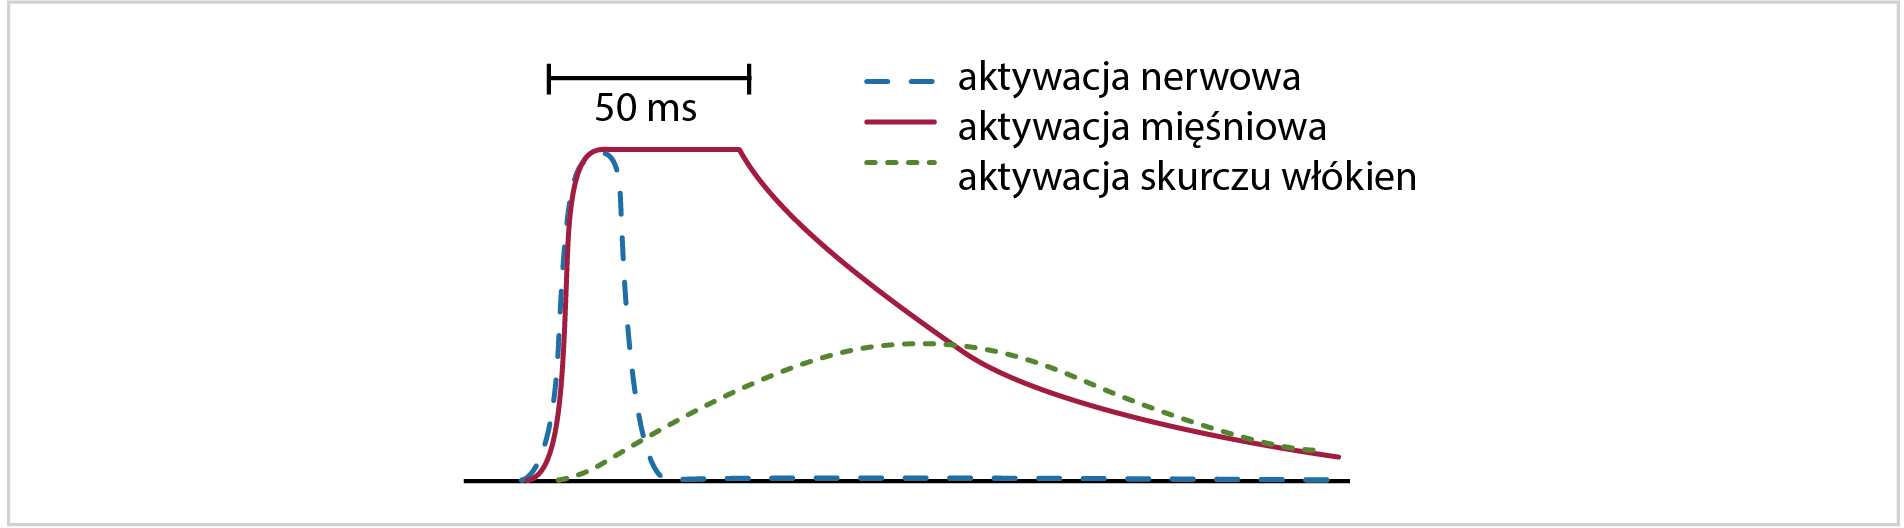
\includegraphics[width=1\textwidth]{figures/skurcz_miesni.png}
	\caption{Schemat generowania skurczu mięśni.}
	\label{muscle-excitements}
\end{figure}

Skurcz mięśni szkieletowych trwa 100--300 milisekund. Schemat czasów i orientacyjnych poziomów poszczególnych aktywacji, przedstawiono na Rys. \ref{muscle-excitements}. Jak wcześniej zaznaczono, siła wygenerowana przez skurcz jest przekazywana za pomocą ścięgien do układu szkieletowego. Dobrym przybliżeniem tego procesu jest \textit{model Hill'a} \cite{Hill1938}. Jego warianty, których przykłady opisane są np. w \cite{Perreault2003} służą obecnie w wielu rozwiązaniach do symulacji pracy układu mięśniowo-szkieletowego. Przykład z popularnego rozwiązania OpenSim rozwijanego na Uniwersytecie Stanforda znajduje się na Rys. \ref{hill-model}.
\begin{figure}[h!]
	\centering
	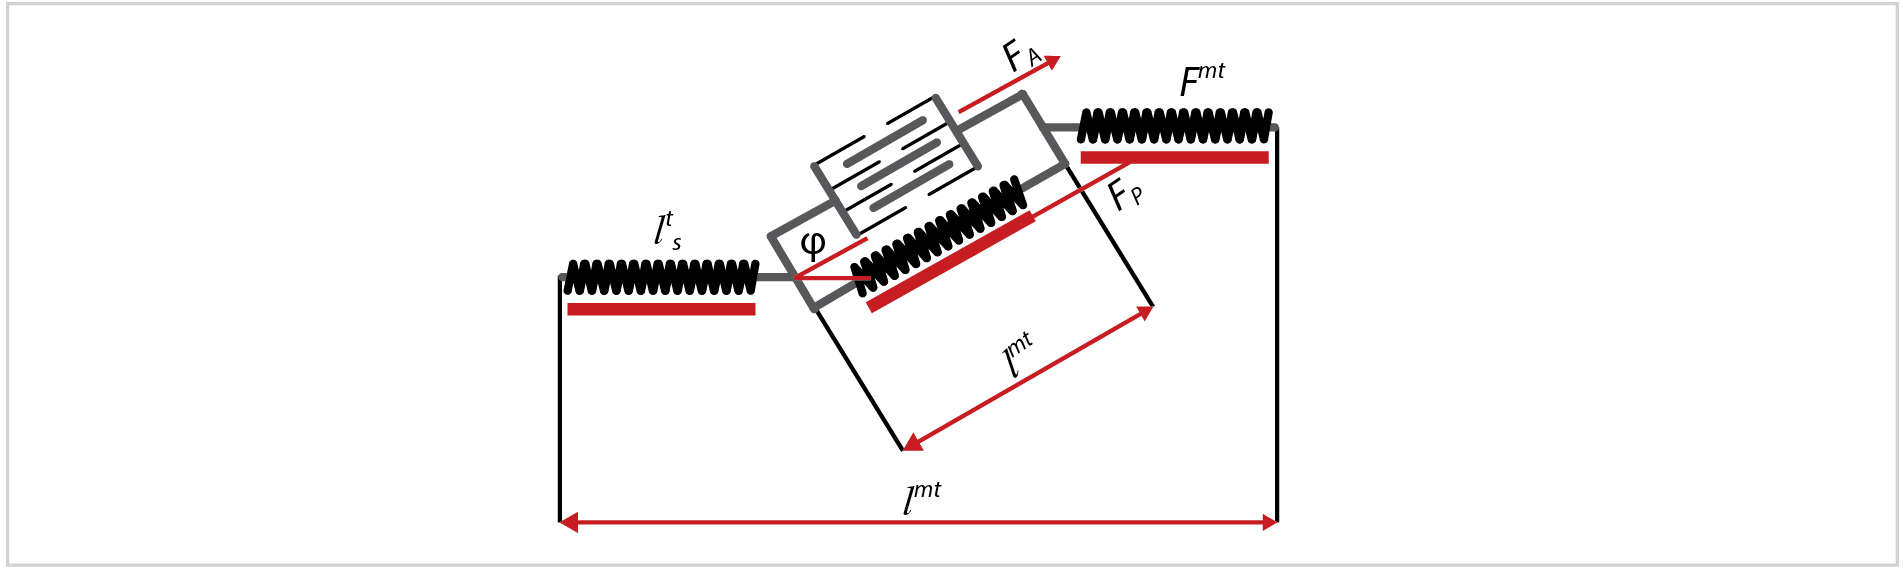
\includegraphics[width=1\textwidth]{figures/Hill.png}
	\caption{Schemat modelu typu Hilla stosowany w oprogramowaniu OpenSim (na podst. \cite{Romero2016}).}
	\label{hill-model}
\end{figure}

Na podanym schemacie $F_A$\index{$F_A$ -- siła wywołana skurczem mięśni} oznacza siłę wywoływaną skurczem mięśni, $F_P$\index{$F_P$ -- pasywna siła odpowiadająca za bezwładność tkanki miękkiej w mięśniu} \linebreak to pasywna siła odpowiadająca za bezwładność tkanki miękkiej w mięśniu, a $F^{mt}$\index{$F^{mt}$ -- wynikowa siła przekazywana przez ścięgno} to wynikowa siła przekazywana przez ścięgno, która zależy od długości ścięgna $l_t$\index{$l_t$ -- długości ścięgna} \linebreak i kąta $\phi$\index{$\phi$ -- kąt pomiędzy ścięgnem a mięśniem} pomiędzy ścięgnem a mięśniem. To właśnie na skutek przekroczenia wartości granicznej siły $F^{mt}$ dochodzi najczęściej do urazu ścięgna Achillesa. 

\subsection{Urazy i czynniki im sprzyjające}
\label{seq:epidemiology}
Uszkodzenie ścięgna Achillesa jest jednym z najczęściej występujących urazów układu mięśniowo-szkieletowego. Przykładowo, dla społeczeństwa amerykańskiego, urazy te występują u 18-tu na 100.000 osób rocznie. Ryzyko ponownego zerwania ścięgna wynosi 20--40\% (zob. \cite{EpidemiologyUS}). 

Można wyróżnić dwa mechanizmy uszkodzenia ścięgna Achillesa: 
\begin{enumerate}[noitemsep,nolistsep]
	\item Uraz bezpośredni, do którego zaliczyć można urazy otwarte spowodowane np. przecięciem ostrym przedmiotem takim jak szkło oraz urazy zamknięte spowodowane nagłym uderzeniem w napięte ścięgno.
	\item Uraz pośredni, znacznie częściej spotykany niż uraz bezpośredni. Powstaje \linebreak on w wyniku nagłego, silnego skurczu mięśnia połączonego często z innymi siłami zewnętrznymi towarzyszącymi np. podczas upadku.
\end{enumerate}
O ile uraz bezpośredni jest najczęściej następstwem nieszczęśliwego wypadku, o tyle urazy pośrednie mają swoją przyczynę w rodzaju wykonywanych czynności oraz predyspozycji danej osoby. 

Zazwyczaj do urazów pośrednich dochodzi podczas uprawiania sportu. Dotyczy to zwłaszcza sportu rekreacyjnego (około 70\% przypadków). W tym obszarze \linebreak aż 75\% przypadków przytrafia się mężczyznom w przedziale wiekowym wahającym się od 30-tego do 50-tego roku życia. Statystyki te mają związek z obniżeniem poziomu ukrwienia ścięgna po 30-tym roku życia oraz sporadycznym, ale nadmiernym obciążaniem ścięgna przez osoby niewytrenowane (zob. \cite{Etiologia}). Ponadto, istotne dane zebrane w duńskim społeczeństwie, przeanalizowane w \cite{Ganestam2015}, pokazują również, że wzrost całościowej liczby przedmiotowych urazów, wynika także z faktu starzenia się społeczeństwa oraz zwiększonej liczby zerwań w grupie wiekowej po 50-tym roku życia. 

Dyscypliny sportowe, podczas których najczęściej dochodzi do urazu ścięgna Achillesa to: piłka nożna, siatkówka, tenis, taniec, koszykówka, skoki, biegi, piłka ręczna, aerobic, pływanie, ping-pong, biegi, narciarstwo, balet. Proporcje są naturalnie uzależnione od popularności danego sportu w konkretnym kręgu ludzi. \linebreak Na Rys. \ref{rupture} zobrazowano udział poszczególnych dyscyplin w urazach ścięgna Achillesa dla społeczeństwa amerykańskiego. 
\begin{figure}[h!]
	\centering
	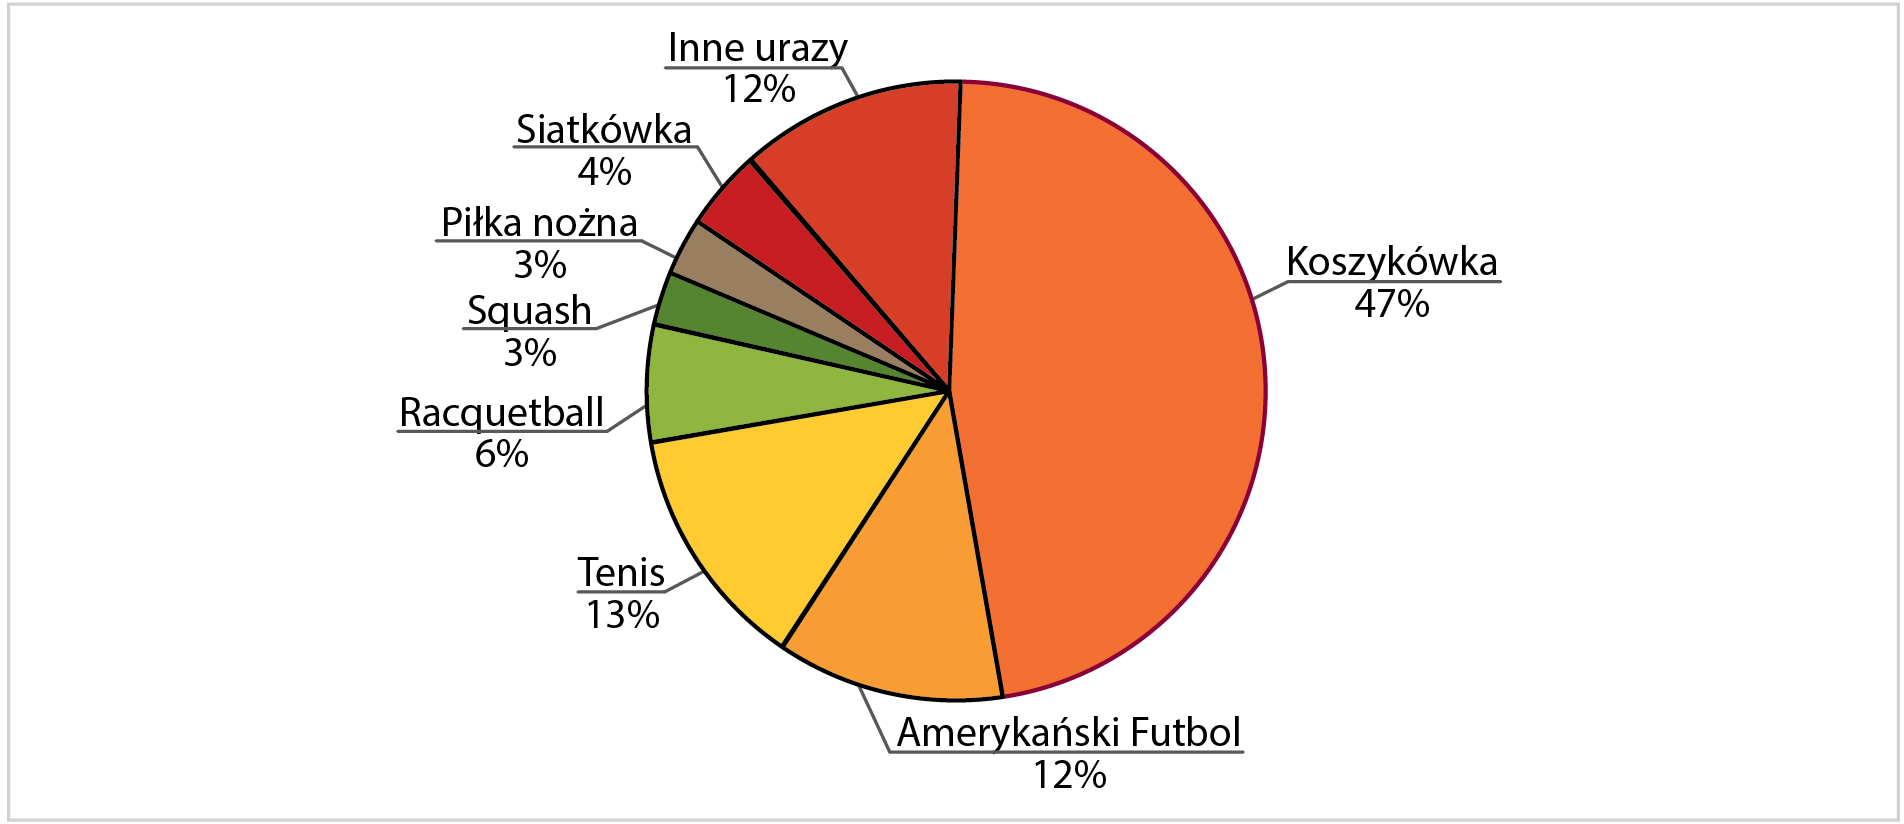
\includegraphics[width=1\textwidth]{figures/Achilles_zerwanie.png}
	\caption{Wykres przedstawiający proporcje występowania urazu ścięgna Achillesa w różnych dyscyplinach sportowych na przykładzie amerykańskiego społeczeństwa (na podst. \cite{EpidemiologyUS}).}
	\label{rupture}
\end{figure}

\newpage
W Stanach Zjednoczonych sportem największego ryzyka jest koszykówka (47\%), natomiast w Europie jest to piłka nożna (około 60\%). Według szacunków przedstawionych w \cite{CHIRALI2014211} uraz ścięgna Achillesa stanowi 5--10\% wszystkich urazów atletycznych.

Powszechnie uważa się, że zdrowe ścięgno piętowe jest bardzo ciężko zerwać \linebreak z uwagi na jego dużą wytrzymałość. Wycinek ścięgna o przekroju 1 cm$^2$ jest w stanie utrzymać masę 500--1000 kg \cite{Maquirriain2011}. Do urazów dochodzi zatem najczęściej, gdy ścięgno jest zmienione patologicznie. Czynniki powodujące osłabienie ścięgna Achillesa można podzielić na: zewnętrzne i wewnętrzne.

Do czynników wewnętrznych należy zaliczyć:
\begin{itemize}[noitemsep,nolistsep]
	\item zmiany degeneracyjne -- inwolucyjne (zwłaszcza przy wieku powyżej 30-tu lat), na podłożu stanów zapalnych (w szczególności przewlekłych), związane z mikrourazami;
	\item nadmierne przeciążenia -- nieprawidłowa aktywność fizyczna;
	\item choroby metaboliczne i układowe -- takie jak np. toczeń trzewny, dna moczanowa, nadczynność tarczycy, gruczolaki przysadki mózgowej, reumatoidalne zapalenie stawów, kolagenozy;
	\item odchylenia anatomiczne i biomechaniczne -- anomalie takie jak: piszczel szpotawa, stopa koślawa, stopa płasko-koślawa, niestabilność stawu skokowego, koślawość lub szpotawość tyłostopia, osłabienie i przykurcz mięśni okołostawowych, ograniczenie ruchomości stawu skokowo-goleniowego i skokowo-piętowego, nierówność kończyn dolnych, nieprawidłowy stereotyp chodu, pogłębione krzywizny kręgosłupa, zespół ciasnoty przedziałów powięziowych w obrębie przedziału tylnego goleni;
	\item zaburzenia naczyniowe -- związane ze schorzeniami takimi jak: hiperlipidemia, cukrzyca lub wywołane nadmiernym paleniem tytoniu;
	\item inne, takie jak: dysbalans mięśniowy, zaburzenia proprioceptywne, niepełne wyleczenie poprzednich obrażeń, przyjmowanie kortykosteroidów.
\end{itemize}

Do czynników zewnętrznych zaliczyć można:
\begin{itemize}[noitemsep,nolistsep]
	\item błędy w metodyce prowadzenia zajęć -- np. nadmierny trening, trening jednostronny, trening wszechstronny z przewagą intensywności nad wytrzymałością czynnościową aparatu więzadłowo-stawowo-mięśniowego, chęć nadrobienia zaległości treningowych;
	\item nagła zmiana dyscypliny sportowej lub aktywności rekreacyjnej;
	\item inne takie jak: nieodpowiednia nawierzchnia, niekorzystne warunki pogodowe, nieodpowiednie obuwie, zbyt krótkie przerwy między zawodami lub treningami.
\end{itemize}

Obecnie ustalenie jednej optymalnej metody leczenia dla każdego rodzaju uszkodzenia ścięgna Achillesa nie jest możliwe. Wybór uwarunkowany jest poziomem \linebreak i stopniem zniszczenia ścięgna, stanem zdrowia pacjenta oraz kwalifikacjami, doświadczeniem i możliwościami danego ośrodka. W kolejnym punkcie omówione zostaną współczesne metody leczenia tego schorzenia, natomiast w Rozdziale \ref{NewMethod} zaprezentowana zostanie nowa metoda monitorowania procesu gojenia się ścięgna Achillesa, która może być wykorzystana do optymalizacji rehabilitacji opisanego problemu. 

\subsection{Fazy gojenia, leczenie i rehabilitacja}
\label{gojenie}

Proces gojenia się ścięgna Achillesa można podzielić na trzy zachodzące na siebie etapy. W pierwszej kolejności dochodzi do stanu zapalnego. Jest to tzw. \textit{faza zapalna} (ang. \textit{inflammatory phase}), która trwa przez pierwszy tydzień gojenia się. Następnie występuje \textit{faza proliferacji} (ang. \textit{proliferative phase}), trwająca od drugiego \linebreak do szóstego tygodnia. Cały proces kończy się \textit{fazą przebudowy} (ang. \textit{remodeling phase}), która może trwać nawet do 18-tego miesiąca po urazie \cite{Sharma2006, Yang2013, Docheva2015, CMC}. 

Faza zapalna zaczyna się od razu po wypadku. W miejscu urazu tworzy się skrzep krwi oraz uwalniane są prozapalne substancje chemiczne, cytokiny, które \linebreak w znaczącym stopniu odpowiadają za proces aktywacji i migracji komórek zapalnych z otoczenia do miejsca zapalenia \cite{Lin2004}. Komórki te, a dokładniej mówiąc leukocyty \linebreak i makrofagi, rozpoczynają \textit{fagocytozę}, czyli proces mający na celu usunięcie obumarłej tkanki oraz skrzepu \cite{Yang2013, Beredjiklian2003, Lin2004}. Symultanicznie dochodzi do aktywacji i selekcji \textit{tenocytów} (komórek ścięgna), które rozpoczynają odbudowę włókien ścięgna \cite{Yang2013} oraz inicjują drugą fazę całego procesu.

W fazie proliferacji poziom komórek zapalnych zaczyna spadać. Czynniki wzrostu, uwalniane m.in. przez makrofagi, nasilają migrację i rozmnażanie tenocytów wokół miejsca urazu. Skutkiem tego procesu jest wytworzenie nowych włókien kolagenu typu III. Nowopowstałe struktury są początkowo zorientowane losowo \cite{Yang2013, Beredjiklian2003, Docheva2015}, dlatego rozpoczyna się trzecia faza mająca na celu odtworzenie struktury zdrowego ścięgna.

W trakcie trwania ostatniej fazy, nazywanej również \textit{remodelingiem}, włókna kolagenu typu III zastępowane są kolagenem typu I. Pod wpływem naprężeń struktura włókien zmienia się i wyrównuje zgodnie z kierunkiem występujących sił \cite{Yang2013}. Włókna pracujące niezgodnie z przewidzianym ruchem ulegają zerwaniu i fagocytozie, \linebreak a te które wspomagają zadany ruch ulegają wzmocnieniu. 

Pomimo całego wyżej opisanego procesu, ścięgno wygojone odbiega strukturą od ścięgna zdrowego. Charakteryzuje się nawet dwukrotnie zwiększoną powierzchnią przekroju poprzecznego oraz podatnością na ponowne zerwania z uwagi na zmniejszoną odporność na obciążenia. 

Uraz ścięgna Achillesa można leczyć zachowawczo lub operacyjnie. Zachowawcze leczenie stosuje się najczęściej przy częściowym uszkodzeniu ścięgna lub u osób, które mają przeciwwskazania do leczenia chirurgicznego. Stosowane jest wówczas unieruchamianie kończyny np. poprzez włożenie w but ortopedyczny lub gips. Dodatkowo można również stosować preparaty z komórek macierzystych i czynników wzrostu \cite{CMC}. Wybór leczenia zachowawczego wiąże się z długotrwałym, trwającym około 10 tygodni unieruchomieniem kończyny przed przystąpieniem do rehabilitacji.

Leczenie operacyjne stosowane jest najczęściej w przypadku uszkodzenia całkowitego. Tuż po urazie lub po przejściu najintensywniejszych procesów fazy zapalnej wykonuje się szycie ścięgna. Stosowane są metody operacji na otwartym ścięgnie lub przezskórnie. Zabieg przezskórny polega na zbliżeniu kikutów ścięgna specjalnym szwem przeprowadzanym przez małe nacięcia. W teorii metoda ta umożliwia szybsze obciążanie nogi po operacji, skraca okres unieruchomienia i umożliwia szybszą rehabilitację. W praktyce chirurgom rzadko jednak udaje się uzyskać jakość zszycia porównywalną z metodą otwartą. 

Rehabilitacja po urazie również podzielona jest ze względu na fazy gojenia. \linebreak W pierwszej fazie terapia skupia się wokół ochrony miejsca urazu, odciążenia nogi, redukcji obrzęku i złagodzenia stanu zapalnego. Dokonuje się również zabiegów mających na celu wczesną mobilizację ścięgna i przywrócenia ślizgu. Ochrona miejsca urazu może być wykonana przez zastosowanie dwuczęściowej łuski gipsowej lub buta ortopedycznego. Redukcję obrzęku wykonuje się np. poprzez masaż limfatyczny. Stan zapalny łagodzony jest chłodzeniem i okładami oraz lekami, natomiast ślizg przykładowo stymuluje się elektrostymulacją oraz mobilizacją mięśni poprzez zginanie stopy.
\newpage
W drugiej fazie zabiegi rehabilitacyjne są kontynuacją działań wykonywanych podczas pierwszej fazy. Szczególny nacisk przewidziany jest na przeciwdziałanie powstawania zrostów poprzez pracę nad ślizgiem ścięgna oraz mobilizacją tkanek miękkich. W szczególności rehabilitanci poświęcają dużo uwagi na ćwiczenia dotyczące mobilizacji blizny i tkanek okalających. Nasilane są również zabiegi elektrostymulacji mające na celu utrzymanie masy mięśniowej oraz ćwiczenia związane ze stabilizacją stawu skokowego takie jak ćwiczenia izometryczne mięśni prostujących i pronujących stopę. W tej fazie stosuje się wciąż ochronę miejsca urazu oraz aplikuje się metody redukcji obrzęku.

Trzeci etap (tj. przebudowa) to najdłuższy z etapów gojenia się tkanek ścięgnistych, podczas którego zachodzi najwięcej zmian w strukturze, odporności ścięgna oraz jego funkcji. W tym okresie można wyszczególnić następujące cele rehabilitacji: 
\begin{itemize}[noitemsep,nolistsep]
	\item przeciwdziałanie zrostom tkanek otaczających Achillesa; 
	\item wzmocnienie mięśni: brzuchatego i płaszczkowatego; 
	\item przywrócenie pełnego zakresu ruchu i kluczowych funkcji ścięgna; 
	\item zwiększenie elastyczności tkanek wokół ścięgna.
\end{itemize}

Oprócz podstawowych zabiegów ochronnych i fizjoterapii do działań włączane \linebreak są terapie związane z ćwiczeniami czynnymi z oporem, stymulujące technikę prawidłowego chodu, ćwiczenia wzmacniające obręcz biodrową, ćwiczenia sensomotoryczne w różnych pozycjach ciała oraz ćwiczenia wzmacniające kończyny dolne na niestabilnym podłożu. Powoli wprowadzane są również aktywności sportowe takie jak rower stacjonarny czy stretching. Celem finalnym tego etapu jest powrót \linebreak do pełnej sprawności. 

Dużą nadzieję wiążę się z nowymi technikami bazującymi na zastrzykach z komórek macierzystych. Ciekawą propozycją wydaje się możliwość budowania biodegradowalnych rusztowań (ang. \textit{scaffold}), implementowanych podczas operacji i wspomagających implementację komórek macierzystych i czynników wzrostu w odpowiednie miejsca \cite{START}.

Do oceny tego rodzaju nowatorskich podejść jak również z uwagi na konieczność optymalizacji istniejących metod rehabilitacji i leczenia urazów ścięgna Achillesa potrzebne jest monitorowanie procesu gojenia. 

\section{Wykorzystanie rezonansu magnetycznego}
\label{RM}
Obserwację gojącej się struktury ścięgna Achillesa umożliwiają techniki stosujące różnego rodzaju fale przenikające ciało ludzkie. Sposób w jaki propaguje się fala tworząc \textit{sygnał} zależny jest od właściwości związanych z ośrodkiem propagacji oraz parametrów fali. Do najistotniejszych należą wyrażana w hercach (w skr. Hz) \textit{częstotliwość}, czyli liczba pełnych cykli drgań w ciągu sekundy, \textit{amplituda} tj. maksymalna wartość sygnału falowego oraz \textit{faza} określająca, w której części cyklu znajduje się sygnał. W technikach obrazowania medycznego wykorzystywana jest interpretacja zdarzeń wynikających ze zmian tych parametrów oraz reagującej materii.

Pierwszą opisaną w tej pracy metodą obrazowania stosowaną do monitorowania gojenia się ścięgna Achillesa jest obrazowanie z wykorzystaniem \textit{Jądrowego Rezonansu Magnetycznego} nazywanego dla uproszczenia \textit{Rezonansem Magnetycznym}, w skrócie \textit{RM}\index{RM -- Rezonans Magnetyczny}. Metoda ta bazuje na odpowiednim odczycie reakcji jąder atomów na stałe pole magnetyczne generowane przez magnesy (zwykle nadprzewodzące), zmienne pole magnetyczne ze składową prostopadłą do osi stałego pola (generowane w dedykowanej do tego zadania cewce) oraz zmienne pole lokalne wytwarzane przez sąsiednie jądra atomowe.

Zrozumienie właściwości jądra atomowego i reakcji na magnetyzację było możliwe dzięki badaniom naukowym z początku XX wieku. Zapewniły one praktyczną możliwość wykorzystania procesów bazujących na zachowaniach obiektów o bardzo małych masach i wymiarach takich jak cząstki elementarne. Jako przykłady można wskazać prace Alberta Einsteina dotyczące ruchów Browna oraz efektu fotoelektrycznego, opis funkcji falowej zaproponowany przez Erwina Shroedingera, badania Nielsa Bohra, które doprowadziły do utworzenia utylitarnego modelu atomu zawierającego poziomy energetyczne, wyprowadzenie reguły nieoznaczoności przez Wernera Heisenberga, czy też opisanie przez Wolfganga Pauliego konfiguracji cząstek elementarnych w atomie. 

W dużej mierze na bazie powyższych prac zdefiniowana została teoria mechaniki kwantowej umożliwiająca między innymi pogłębienie wiedzy na temat magnetycznej natury składników jądra atomowego tj. \textit{protonów} i \textit{neutronów}. Pierwszy ważny przełom nastąpił w 1933 r., kiedy to Frisch i Stern w \cite{Frisch1933} opisali moment magnetyczny protonu. Rok później, w \cite{Breit1934} Breit i Rabi zaproponowali metodę rezonansową obserwacji właściwości magnetycznych jąder atomowych. W 1946 praca ta została udoskonalona i wykorzystana przez Felixa Blocha do badania cząstek w wodzie \linebreak i parafinie \cite{Bloch1946}. W końcu dzięki pracom m.in. Lautenrbur'a \cite{LAUTERBUR1973} i Mansfield'a \cite{Mansfield1977} rozwinęły się metody lokalizacji przestrzennej powyższych zmian właściwości magnetycznych, co umożliwiło utylitarną prezentację wizualną wyników. 

Opisując dokładniej to zagadnienie należy zwrócić uwagę na główną właściwość jądra atomowego umożliwiającą działanie RM, czyli \textit{spin}. Tylko jądra o nieparzystej liczbie masowej posiadają niezerowy spin w stanie podstawowym. Liczba masowa jest sumą liczb protonów i neutronów (por. \cite{RM2015}). Dla przykładu jądro wodoru składające się z jednego protonu spełnia powyższy warunek. 

Umieszczone w polu magnetycznym jądra atomowe posiadające spin wykonują ruch wirowy zwany \textit{precesją}. Częstotliwość tej precesji jest proporcjonalna do natężenia pola magnetycznego i opisana jest \textit{równaniem Larmora} \ref{MRLarmor}:
\begin{equation}
\label{MRLarmor}
\omega_0 = \gamma \ast B_0,
\end{equation}
gdzie $\omega_0$\index{$\omega_0$ -- częstość kołowa protonów} to częstość kołowa protonów, $f_l = \omega_0/2\pi$ to tzw. \textit{częstotliwość Larmora}\index{$f_l$ -- częstotliwość Larmora}, $\gamma$\index{$\gamma$ -- współczynnik żyromagnetyczny właściwy dla danego jądra atomowego} to współczynnik żyromagnetyczny właściwy dla danego jądra atomowego, $B_0$\index{$B_0$ -- wartość indukcji danego pola magnetycznego} \linebreak to wartość indukcji danego pola magnetycznego. Dla przykładu częstotliwość Larmora dla jądra wodoru, gdzie $\gamma$=42,57 MHz/T dla pola 1,5 T równa jest 63,8 MHz. 

Jądra atomowe o niezerowym momencie magnetycznym, na skutek działania silnego pola magnetycznego, ulegają swego rodzaju uporządkowaniu. Dodatkowo istotne jest, że jądra o spinach ustawionych równolegle do pola magnetycznego mają mniejsze energie, a o ustawionych antyrównolegle większe. Jądra odchylone impulsami fal elektromagnetycznych od pierwotnego kierunku magnetyzacji rotują \linebreak z częstością Larmora. W przeciętnym wycinku ciała ludzkiego jest znacząco więcej jąder o ustawieniu równoległym niż antyrównoległym. Przykładowo, w stosunkowo niewielkim w porównaniu z wymiarami typowo obrazowanych struktur anatomicznym kawałku o objętości 1 $\times$ 1 $\times$ 5 mm, różnica to około 2 $\times$ $10^{15}$ jąder w polu \linebreak o indukcji 1,5 T. 

Sygnał RM pochodzi od różnicy magnetyzacji jąder ustawionych równolegle \linebreak i antyrównolegle (różnicę tę oznaczamy jako $M_0$\index{$M_0$ -- całkowita magnetyzacja} -- tj. całkowita magnetyzacja). Wyjściowo $M_0$ ma większą wartość zgodną ze zwrotem pola magnetycznego, czyli tzw. \textit{magnetyzację podłużną}. Kierunek prostopadły do magnetyzacji podłużnej nazywany jest \textit{magnetyzacją poprzeczną}.

Zmianę $M_0$ wykonuje się przy pomocy odpowiednio sterowanej cewki nadającej impulsy o częstotliwości fal radiowych (tzw. \textit{impulsy RF} -- od ang. \textit{Radio Frequency}). Impuls RF\index{Impuls RF -- impuls o odpowiedniej częstotliwości fal radiowych} jest krótkotrwały i ma taką samą częstotliwość co częstotliwość precesji. Dzięki temu zachodzi zjawisko \textit{rezonansu magnetycznego}, czyli wymiany energii między jądrami atomowymi a falą radiową. Jądro atomowe pochłania wówczas energię \textit{fotonu} (tj. nośnika oddziaływania elektromagnetycznego) i uzyskuje wyższy poziom energetyczny, odchylając wektor magnetyzacji i zaburzając tym samym uporządkowanie. Następuje zmniejszenie $M_0$ w kierunku podłużnym oraz wzrost magnetyzacji poprzecznej. Po wyłączeniu impulsu RF magnetyzacja wraca do wartości początkowej. 

Istotnymi stałymi w tym procesie są $T2$\index{$T2$ -- czas potrzebny na $e$-krotne obniżenie magnetyzacji poprzecznej}, czyli czas potrzebny na $e$-krotne obniżenie magnetyzacji poprzecznej oraz $T1$\index{$T1$ -- czas po jakim magnetyzacja podłużna wraca do (1 - 1/$e$) początkowej wartości} tj. czas po jakim magnetyzacja podłużna wraca do (1 - 1/$e$) początkowej wartości. Z reguły T2 $\leq$ T1, a zawsze T2 $\leq$ 2T1.   

Lokalizacja zmian magnetyzacji w poszczególnych \textit{wokselach} (tj. wycinkach przestrzeni 3D o określonych wymiarach) odbywa się przy pomocy celowanego różnicowania fazy i częstotliwości wektorów magnetyzacji. Operacja ta wykonywana jest przy pomocy sygnału z dodatkowych cewek gradientowych. Wartości w warstwie, \linebreak w której dokonywany jest pomiar, kodowane są przy pomocy nałożenia na pole $B_0$ pola gradientowego $G_{zz}$\index{$G_{zz}$ -- wartość pola gradientowego w kierunku $z$}, co umożliwia wzbudzenie jąder atomowych w tych wokselach, dla których współrzędna $z$\index{$z$ -- trzecia  współrzędna prostokątna} wyraża się wzorem:
\begin{equation}
\Delta z = \frac{\Delta \omega}{\gamma G_{zz}},
\end{equation}
gdzie $\Delta \omega$\index{$\Delta \omega$ -- szerokość widmowa pobudzającego jądra impulsu RF} to szerokość widmowa pobudzającego jądra impulsu RF. Współrzędna \linebreak $y$\index{$y$ -- druga współrzędna prostokątna} kodowana jest przy pomocy zróżnicowania fazy rotujących w różnych obszarach wektorów magnetyzacji na skutek działania pola gradientowego $G_{yz}$\index{$G_{yz}$ -- wartość pola gradientowego w kierunku $y$} -- tzw. \textit{gradientu kodowania fazy}. Zróżnicowanie fazy wyraża się wzorem:
\begin{equation}
\phi = \gamma G_{yz}yT_{y},
\end{equation}
gdzie $T_y$\index{$T_y$ -- czas włączenia pola gradientowego $G_{yz}$} oznacza czas włączenia pola gradientowego $G_{yz}$. Ostatecznie, współrzędna $x$\index{$x$ -- pierwsza współrzędna prostokątna} kodowana jest w wyniku zróżnicowanie częstości precesji wektorów magnetyzacji poprzez włączanie pola gradientowego $G_{xz}$\index{$G_{xz}$ -- wartość pola gradientowego w kierunku $x$} (zob. \cite{ObrazowanieMedyczne}). 

Nieprzetworzona informacja z wokseli o współrzędnych $x$, $y$, $z$ nazywana jest \textit{przestrzenią K} i koduje ona składniki częstotliwości sygnału RM. Do transformacji \linebreak z przestrzeni częstotliwości na przestrzeń obrazu używana jest operacja matematyczna zwana \textit{odwrotną transformacją Fouriera}. Przykład takiego działania można znaleźć w \cite{Q&AinMRI}.

Główną informacją jaką otrzymujemy za pomocą obrazowania metodą jądrowego rezonansu magnetycznego jest rozkład gęstości jąder atomowych o niezerowym spinie. Jądra wodoru mają największy spośród jąder atomowych współczynnik żyromagnetyczny oraz występują w znaczącej liczbie w prawie każdej z tkanek ludzkich (por. \cite{RM2015}), dlatego ich rozkład jest najczęściej mierzony. Jedynie w szczególnych przypadkach stosuje się obrazowanie z wykorzystaniem częstotliwości rezonansu odpowiednich dla innych pierwiastków takich jak fosfor \cite{Sun2016}, sód \cite{Summers1991} czy węgiel \cite{Dria2002}. 

Dodatkowo, obserwacja zmiany sygnału RM w czasie często dostarcza istotnych danych na temat właściwości fizyko-chemicznych struktur anatomicznych. W szczególności uzyskanie informacji na temat parametrów $T1$ i $T2$ zapewnia możliwość różnicowania tkanek. Z uwagi na ten fakt, dla uwydatnienia interesujących informacji, stosuje się szereg ustawień urządzeń do rezonansu magnetycznego pogrupowanych w \textit{sekwencje RM} oraz ich podgrupy nazywane w tej pracy \textit{modalnościami}. \linebreak Do badań opisanych w dalszej części tego manuskryptu zostało użytych 7 sekwencji, w tym jedna z 4 modalnościami. Zostaną one pokrótce scharakteryzowane poniżej:
\begin{itemize}[noitemsep,nolistsep]
	\item \textit{T1 zależne} -- zależność sygnału rezonansu magnetycznego $MR_s$\index{$MR_s$ -- wartość sygnału rezonansu magnetycznego $MR_s$} w tej sekwencji opisana jest w następujący sposób: 
	\begin{equation}
		MR_s \sim \gamma_{pd} \ast [1-e^{-TR/T1}],
	\end{equation}
	gdzie $\gamma_{pd}$\index{$\gamma_{pd}$ -- gęstość protonowa tkanki} to gęstość protonowa tkanki, a $T1$ odpowiada momentowi, gdy wartość magnetyzacji podłużnej wynosi 63\% wartości początkowej. Czas ten nie jest znany, stąd użytkownik określa \textit{czas repetycji} $TR$\index{$TR$ -- czas repetycji} rzędu spodziewanego czasu $T1$.
	\item \textit{T2 zależne} -- zależność sygnału rezonansu magnetycznego $MR_s$ w tej sekwencji opisana jest w następujący sposób: 
	\begin{equation}
	\label{T2ecquation}
	MR_s \sim \gamma_{pd} \ast e^{-TE/T2}.
	\end{equation}
	$T2$ odpowiada momentowi, gdy wartość magnetyzacji poprzecznej wynosi 37\% wartości początkowej. Podobnie jak w poprzedniej sekwencji, czas ten nie jest znany, więc użytkownik określa parametr $TE$\index{$TE$ -- czas echa}, \textit{czas echa}, rzędu czasu $T2$. Sekwencja T2 zależne charakteryzuje się odmienną skalą szarości niż T1 zależne.
	\item \textit{PD}\index{PD -- skrót od ang. Proton density} (od ang. \textit{Proton Density}) -- obraz rekonstruowany na podstawie sygnału RM przy bardzo krótkim $TE$ i bardzo długim $TR$. Wówczas sygnał jest wprost proporcjonalny do $\gamma_{pd}$:
	\begin{equation}
	MR_s \sim \gamma_{pd}.
	\end{equation}
	\item \textit{T2 mapping} -- w tej sekwencji wartość sygnału RM zależna od $T2$ (zob. \ref{T2ecquation}) mierzona jest dla 8 $TE$. Pozwala to na wyliczenie czasu $T2$ (zob. \cite{Regulski2017}).
	\item \textit{T2$^\ast$ GRE} (od ang. \textit{Gradient Echo}) -- jest to przykład \textit{sekwencji gradientowych}, gdzie spin obracany jest za pomocą impulsów RF o mniej niż 90$^\circ$ oraz brak jest kompensacji niejednorodnego pola magnetycznego. Zabieg ten używany jest w celu przyspieszenia pomiaru kosztem jakości sygnału. Stąd też oznaczenie czasu $T2$$^\ast$ $<$ $T2$. 
	\item \textit{T2$^\ast$ GRE TE\_MIN} (od ang. \textit{Minimal Time Echo}) -- obraz rekonstruowany jest na podstawie sygnału RM dla T2$^\ast$  przy minimalnym czasie $TE$ i tylko dla fragmentu przestrzeni K. Zabieg ten skraca znacząco czas badania.
	\item \textit{3D FSPGR}\index{FSPGR -- skrót od ang. Fast Spoiled Gradient Echo} (od ang. \textit{Three-dimensional Fast Spoiled Gradient Echo}) -- jest to szybka sekwencja gradientowa z usuwaną (ang. \textit{spoiled}) pozostałością magnetyzacji poprzecznej. W wyniku sekwencji impulsów RF otrzymywane są 4 modalności: 
	\begin{itemize}[noitemsep,nolistsep]
		\item \textit{In Phase Ideal} -- sygnał mierzony w czasie, gdy protony należące do tłuszczu i wody są w zgodnej fazie;
		\item \textit{Out Phase Ideal} -- sygnał mierzony w czasie, gdy protony należące \linebreak do tłuszczu i wody są w antyfazie;
		\item \textit{Fat Ideal} -- sygnał mierzony przy maksymalnej wartości sygnału od protonów tłuszczu i minimalnej od protonów wody;
		\item \textit{Water Ideal} -- sygnał mierzony przy maksymalnej wartości sygnału \linebreak od protonów wody i minimalnej od protonów tłuszczu.
	\end{itemize}
	Powyższe modalności są możliwe do realizacji, gdyż w sekwencji 3D FSPGR sygnał RM odczytywany jest przy dwóch różnych czasach $TE$. Przy czym czasy $TE$ są tak dobrane, aby sygnały od wody i tłuszczu wzmacniały się (In Phase Ideal) lub osłabiały (Out Phase Ideal). Jest to możliwe, gdyż przy zadanym polu magnetycznym częstotliwość Larmora wodoru w wodzie jest minimalnie inna niż w tłuszczach (fakt ten nazywany jest również przesunięciem chemicznym i jest wykorzystywany w spektroskopii NMR \cite{lide2006crc}). Modalności Water Ideal i Fat Ideal są odpowiednią kombinacją liniową dwóch wcześniejszych -- taką, aby zminimalizować wpływ tłuszczu (Water Ideal) lub wody (Fat Ideal) na sygnał RM.
\end{itemize}

Rezonans magnetyczny może być wykorzystany do monitorowania gojenia się ścięgien i więzadeł, gdyż tkanki miękkie człowieka zawierają dużo atomów wodoru. W kontekście ścięgna Achillesa, RM w szczególności pozwala radiologom na obserwację: ciągłości ścięgna w płaszczyźnie strzałkowej (ang. \textit{sagittal plane}); uszkodzeń śródścięgnistych objawiających się przerwaniem w naturalnym warkoczu ułożonym \linebreak z tkanek; pogrubienia ścięgna ocenianego w przekrojach poprzecznych (ang. \textit{axial planes}); jednorodności, wrzecionowatości i innych nieregularności kształtu; ostrości ścięgna i jego rozgraniczenia od tkanek otaczających wraz ze zmianami występującymi \linebreak na brzegach; obrzęku w okalających ścięgno tkankach; jednorodności charakteryzującej się podobieństwem przekrojów sąsiednich oraz liczby ewentualnych zrostów. Na Rys. \ref{sagittalAchillesComp} zobrazowano zestawienie wykorzystanych w pracy sekwencji, porównując płaszczyzny strzałkowe z widoczną strukturą ścięgna Achillesa.  
\begin{figure}[]
	\centering
	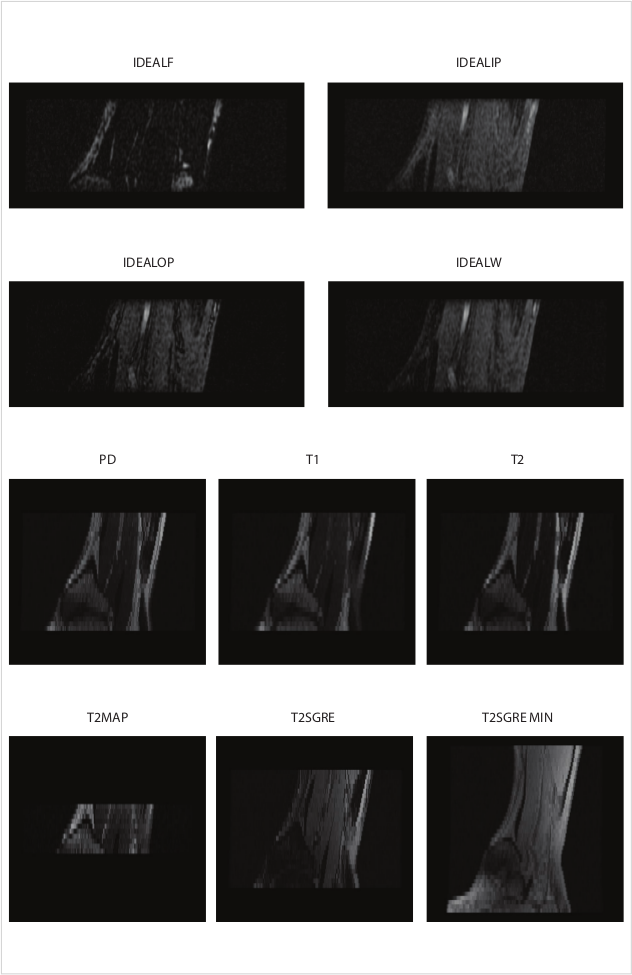
\includegraphics[width=1\textwidth]{figures/sciegno.png}
	\caption{Porównanie sekwencji RM w płaszczyźnie strzałkowej z widoczną strukturą ścięgna Achillesa.}
	\label{sagittalAchillesComp}
\end{figure}

W praktyce radiologicznej bardzo często wykorzystywana jest sekwencja PD obrazująca gęstość wodoru. Jasność na obrazie PD obszarów Achillesa skorelowana jest z uwodnieniem tkanek oraz obecnością mięśni, mniej z tłuszczem, który w niewielkim stopniu występuje w podudziu. Widoczne ciemniejsze pionowe struktury to (od lewej): kość strzałkowa, kość piszczelowa i ścięgno Achillesa. Sekwencja T1 pokazuje podobny rozkład przestrzenny jasności. Jest to spowodowane niewielka ilością tkanki tłuszczowej. Czas relaksacji T1 tkanki tłuszczowej jest znacząco krótszy niż dla większości pozostałych tkanek organizmu, dlatego tkanka tłuszczowa byłaby wyróżniona na jasno (przy czym im krótszy czas T1 tym jaśniejszy obraz). Ścięgno Achillesa w tej sekwencji jest mniej wyszczególnione niż w przypadku PD. Z kolei sekwencja T2 pokazuje większy kontrast -- wyraźnie ciemniejsze kości i ścięgno. Ostatnie jest spowodowane wyjątkowo krótkim czasem relaksacji T2 dla zdrowego ścięgna (rzędu 5 ms, w porównaniu do 2000 ms dla wody). Dlatego sekwencje oparte na czasach T2 są z reguły bardzo przydatne w ocenie stanu ścięgna, w szczególności implikacji jego uwodnienia. Widać to również w przykładach sekwencji T2$^\ast$GRE i T2$^\ast$GRE TE\_MIN będącymi modyfikacjami sekwencji T2, gdzie mierzony jest czas T2$^\ast$, a ponadto są to sekwencje gradientowe. W porównaniu do sekwencji T2 charakteryzują się większą ilością artefaktów lecz pozwalają obrazować tkanki o krótszych czasach relaksacji. Druga z wymienionych sekwencji -- o bardzo krótkich -- nawet rzędu kilku ms. Jak widać, struktury na innych sekwencjach widoczne jako ciemne stają się na tych obrazach jaśniejsze, oznacza to że sekwencje te lepiej od pozostałych różnicują tkanki o bardzo krótkich czasach T2. W szczególności największe widoczne ciemne obszary to ścięgno Achillesa oraz obszary o niewielkiej ilości wodoru (powietrze i kości nie zawierające szpiku kostnego). Modalności należące do sekwencji 3D FSPGR ukazują odpowiednio: uwodnienie (Water Ideal), tłuszcz jako ciemny obszar (Fat ideal) oraz granicę tłuszczu i wody In$/$Out Phase ideal. Z powodu małej ilości tłuszczu w obrazowanym obszarze sekwencja ta ma znikome zastosowanie.

W podsumowaniu należy również powiedzieć o ogólnych ograniczeniach związanych ze stosowaniem RM, wynikających głównie z oddziaływania silnego pola magnetycznego na przedmioty z nim reagujące np. ferromagnetyki zawarte w odłamkach metalowych; urządzenia elektryczne typu wszczepiony stymulator serca lub duże kawałki metalu jak endoprotezy, które mogą się rozgrzać na skutek indukowanych prądów. Wrażliwość pacjenta na hałas lub skłonności klaustrofobiczne również są wskazaniami do wykluczenia z badania. Ponadto urządzenie do rezonansu magnetycznego jest bardzo drogie, nieprzenośne i wymagające specjalnego otoczenia pracy. W celu wyeliminowania tych ograniczeń można posłużyć się inną metodą obrazowania medycznego opisaną w kolejnej sekcji. 

\section{Wykorzystanie ultrasonografii}
\label{USG}

Kolejną z metod obrazowania medycznego jest \textit{Ultrasonografia}, w skr. \textit{USG}\index{USG -- Ultrasonografia} (ang. \textit{Ultrasonography}, \textit{US}). Bazuje ona na efektach związanych z propagacją w tkankach \textit{ultradźwięków} tj. fal akustycznych o częstotliwościach powyżej 20 kHz. W praktyce, z uwagi na parametry związane z rozdzielczością obrazu, są to fale o częstotliwości rzędu kilku MHz, w szczególnych przypadkach kilkudziesięciu.

Propagacja fal akustycznych w przyrodzie była tematem rozważań myślicieli takich jak Pitagoras, Arystoteles czy Galileusz, którzy ugruntowali pole badań pod kolejne osiągnięcia matematyczno-inżynieryjne. W tej kwestii, do jednego z przełomów doszło w 1822 roku, kiedy to szwajcarski inżynier Daniel Colladen oraz matematyk Charles-Francois Sturm wyznaczyli przybliżoną prędkość rozchodzenia się fali akustycznej w wodzie. Badanie wykonano na Jeziorze Genewskim symultanicznie mierząc czas jaki potrzebny był dźwiękowi podwodnego wystrzału i sygnałowi dzwonka rozchodzącego się w powietrzu do przebycia drogi pomiędzy dwoma łódkami oddalonymi o 10 mil. Wyliczona wartość wyniosła wówczas 1435 m/s nie różniąc się znacząco od dzisiaj przyjmowanej estymacji równej 1480 m/s. Analogicznie, stosując nowoczesne techniki, wyliczane są obecnie prędkości rozchodzenia się fali \linebreak w innych ośrodkach takich jak powietrze, tkanki miękkie, kości itp.

58 lat po eksperymencie na Jeziorze Genewskim, w 1880 roku bracia Curie opisali w \cite{Curie1880} \textit{efekt piezoelektryczny}, czyli zjawisko polegające na pojawieniu się ładunku elektrycznego pod wpływem naprężeń mechanicznych w krysztale o anizotropowej budowie, takiej jak ma np. kwarc. W przypadku odwrotnym, przyłożenie napięcia do odpowiedniego kryształu generuje drgania (tzw. \textit{odwrotny efekt piezoelektryczny}). 

Efekty te są wykorzystywane w \textit{głowicy aparatu usg}, przyrządu do generowania \linebreak i odbierania ultradźwięków. Przykładowo, polaryzowanie kryształu piezoelektrycznego krótkim impulsem elektrycznym $\sigma_1(t)$\index{$\sigma(t)$ -- wartość impulsu elektrycznego} pobudza go do drgań na własnej \textit{częstotliwości rezonansowej}. Zakładając, że ów kryształ ma kształt walca o grubości $d$=0,64 mm\index{$d$ -- grubość np. walca}, to będzie stanowił rezonator półfalowy, w którym wystąpi drganie rezonansowe o długości fali $\lambda = 2d$ czyli $\lambda = 1,28$ mm\index{$\lambda$ -- długość fali}. Jeżeli wykonany jest z tytanianu baru, dla którego prędkość propagacji drgań wynosi $c$=4460 m/s\index{$c$ -- prędkość propoagacji drgań}, to częstotliwość drgań własnych tego kryształu wyniesie:
\begin{equation}
f = \frac{c}{\lambda} = \frac{4460 m/s}{1,28 mm} = 3,5 \; MHz.
\end{equation}
Odwrotnie, powracająca fala tzw. \textit{echo} wygeneruje impuls elektryczny $\sigma_2(t)$ wskutek drgań wywołanych w krysztale. Echo jest falą różniącą się od sygnału nadawanego, a zmiany te są w przeważającym stopniu efektem zjawisk takich jak: \textit{odbicia}, \textit{załamania}, \textit{dyfrakcja}, \textit{rozpraszanie} i \textit{pochłanianie} (zob. \cite{makarewicz1978}).

Zjawiska te zależą od częstotliwości fali, która propaguje się w ośrodku o pewnej \textit{impedancji akustycznej ośrodka} $Z$\index{$Z$ -- impedancja akustyczna ośrodka} wyrażanej jako:
\begin{equation}
Z = \rho c = \sqrt{\epsilon \rho},
\end{equation}
gdzie $c$, to prędkość rozchodzenia się fali, $\rho$\index{$\rho$ -- gęstość ośrodka} to gęstość ośrodka, a $\epsilon$\index{$\epsilon$ -- moduł odkształcalności objętościowej} to \textit{moduł odkształcalności objętościowej}, tj. parametr opisujący jak zmieni się objętość ośrodka pod danym ciśnieniem. Parametry wybranych ośrodków zestawiono w Tabeli \ref{tab:USG-params}.
\vspace{10px} 
\renewcommand{\arraystretch}{1.2}
\begin{table}[h!]
	\setlength{\tabcolsep}{14pt}
	\centering
	\caption{Parametry ośrodków często mierzonych w badaniach USG.}
	\scriptsize
	\label{tab:USG-params}
	\begin{tabular}{l | l | l | l | l }
		%\hline
		Ośrodek  & Moduł sprężystości  & Gęstość  & Prędkość  & Impedancja akustyczna  \\  
		& [kg/m/s$^2\times10^{-8}$] & [kg/m$^3$] & [m/s] & [kg/m$^2$/s$^2\times10^{-8}$] \\ \hline \hline
		Powietrze   & 0,0000134 & 1,2 & 330 & 0,0004 \\ \hline
		Woda (20$^\circ$ C) & 2,19 & 1000 & 1480 & 1,48  \\ \hline
		Tkanki miękkie & 2,51 & 1060 & 1540 & 1,63  \\ \hline
		Tkanka tłuszczowa & 2,0 & 952 & 1450 & 1,38  \\ \hline
		Wątroba & 2,54 & 1060 & 1550 & 1,64  \\ \hline
		Mięśnie wzdłużne & 2,74 & 1080 & 1592 & 1,70  \\ \hline
		Mięśnie poprzecz. & 2,80 & 1080 & 1610 & 1,74  \\ \hline
		Mózg & 2,40 & 994 & 1550 & 1,55  \\ \hline
		Śledziona & 2,59 & 1045 & 1578 & 1,64  \\ \hline
		Krew & 2,47 & 1057 & 1057 & 1,62  \\ \hline
		Kość & 32,0 & 1912 & 4080 & 7,8  \\ \hline
		Płuca & 0,169 & 400 & 650 & 0,26  \\ \hline
	\end{tabular}
\end{table}
\renewcommand{\arraystretch}{1}

Dla przykładu, do zjawiska załamania lub odbicia dochodzi kiedy fala pada \linebreak na granicę dwóch ośrodków o różnych impedancjach akustycznych $Z_1$ i $Z_2$. Dla fali prostopadłej zależność ta opisana jest następująco:
\begin{equation}
R = \frac{I_r}{I_0} = \left(\frac{Z_1-Z_2}{Z_1+Z_2}\right)^2,
\end{equation}
gdzie $I_r$\index{$I_r$ -- natężenie fali padającej} to natężenie fali padającej, a $I_0$\index{$I_0$ -- natężenie fali padającej} odbitej. Natomiast $R$\index{$R$ -- energetyczny współczynnik odbicia}, czyli energetyczny współczynnik odbicia, jest parametrem, który rośnie wraz ze wzrostem kąta odchylenia od kierunku prostopadłego, aż do całkowitego odbicia.

Z kolei do rozpraszania bądź pochłaniania fali dochodzi kiedy to fala pokonuje daną drogę w ośrodku o pewnej $Z$, co zapisywane jest następująco:
\begin{equation}
I=I_0 \epsilon^{-\gamma x},
\end{equation}
gdzie $\gamma$\index{$\gamma$ -- współczynnik osłabienia fali} to współczynnik osłabienia zależny od $Z$, a $x$\index{$x$ -- droga przebyta przez falę} to droga przebyta przez falę. Efekt ten można korygować poprzez dobór odpowiedniego $I_0$ lub mierząc czas powrotu i na tej podstawie wyliczając spodziewane osłabienie. Zabieg ten pozwala obrazować jednocześnie struktury położone na rożnych głębokościach.

Analiza amplitudy i częstotliwości sygnału nadanego i echa umożliwia rekonstrukcję obrazu USG. W przypadku najczęściej stosowanych w praktyce rekonstrukcji przekrojów dwuwymiarowych (tzw. \textit{tryb B}) współczesny tor budowania prezentacji wizualnej (tzw. \textit{beamforming}) wygląda następująco: 
\begin{enumerate}[noitemsep,nolistsep]
	\item Głowica ultradźwiękowa emituje impulsy w postaci wąskiej wiązki w ściśle określonym kierunku. Wiązka jest efektem interferencji sygnału z $N$ przetworników zawierających kryształy piezoelektryczne.
	\item Echa z danego kierunku pozwalają na obliczenie pojedynczego promienia akustycznego, który jest ilorazem charakterystyk nadawanego i odbieranego sygnału.
	\item Wszystkie promienie, których we współczesnych aparatach może być do kilkuset (zob. \cite{GEVoluson}), służą do formowania obrazu, który tworzony jest we \textit{współrzędnych biegunowych} ($r$, $\theta$) w przypadku głowic mechanicznych sektorowych, wieloelementowych convex czy fazowych lub we współrzędnych prostokątnych ($x$, $y$) w przypadku głowic mechanicznych lub wieloelementowych liniowych. 
\end{enumerate}

Tryb B umożliwia również wizualizację obrazów dynamicznych. Przykładowo, jeżeli na obraz składa się 400 promieni i każdy odsłuchiwany jest do głębokości 15 cm, to czas gromadzenia danych dla ośrodka o średnim c=1500 m/s wynosi $2\frac{2\times15}{1500 m/s}\times400 = 0,08$ s, czyli 12 obrazów na sekundę. Częstotliwość tę można zwiększać zmniejszając liczbę promieni lub głębokość obserwacji.

Innym często stosowanym trybem rekonstrukcji obrazu jest \textit{tryb D} bazujący \linebreak na \textit{efekcie Dopplera}, do którego dochodzi w przypadku odbicia fali od ośrodka przesuwającego się względem głowicy. Zmienia się wówczas częstotliwość fali, co wyrażone jest następującym wzorem:
\begin{equation}
f_r = 2 f_o\frac{v}{c}\cos(\theta),
\end{equation} 
gdzie $f_0$\index{$f_0$ -- częstotliwość fali nadawanej} to częstotliwość fali nadawanej.  $f_r$\index{$f_r$ -- różnica pomiędzy częstotliwością odbieraną i emitowaną przez głowicę USG} to różnica pomiędzy częstotliwością odbieraną i emitowaną przez głowicę USG. Kąt $\theta$\index{$\theta$ -- kąt pomiędzy kierunkiem propagacji fali ultradźwiękowej i kierunkiem prędkości poruszającego się ośrodka} jest kątem pomiędzy kierunkiem propagacji fali ultradźwiękowej i kierunkiem prędkości poruszającego się ośrodka. $v$\index{$v$ -- prędkość ośrodka} i $c$\index{$c$ -- prędkość dwięku w ośrodku} natomiast to odpowiednio prędkości ośrodka i dźwięku w ośrodku.

Dla przykładu, im większa prędkość komórek przesuwających się w monitorowanym ciele pacjenta, tym większa jest $f_r$. Dlatego tryb D z powodzeniem jest wykorzystywany np. do monitorowania przepływu krwi w dużych naczyniach takich jak tętnice.

Rozwinięciem trybu D jest tryb \textit{Power D}\index{Power D -- Power Doppler} (od ang. \textit{Power Doppler}). W tym trybie zamiast przesunięcia częstotliwości interpretowana jest moc sygnału dopplerowskiego. Za pomocą odpowiedniego parametru nazywanego \textit{gain} można wzmacniać sygnał Power D uwidaczniając np. informacje pochodzące od przepływów krwi z niewielką prędkością w charakteryzujących się małą średnicą naczyniach krwionośnych. Jest to również możliwe, gdyż tryb Power D ma nawet trzykrotnie większą czułość niż standardowy tryb D \cite{Babcock1996}. Wynika to z faktu, że Power D nie uwzględnia informacji o prędkości czy kierunku przepływów, a jest sumą wszystkich możliwych przesunięć częstotliwości w zadanym fragmencie obrazowanego obiektu.

W kontekście ścięgna Achillesa tryb Power D może służyć do oceny unaczynienia ścięgna w kolejnych etapach gojenia, które jak wiadomo z p. \ref{gojenie} zmienia się w czasie. Tryb B natomiast może być użyteczny do obrazowania struktury tkanek miękkich. W praktyce wykorzystywana jest zwłaszcza możliwość zobrazowania ukierunkowania struktur włókien ścięgnistych na podstawie czego radiolog może wnioskować o fazie gojenia (zob. Rys. \ref{usgAchillesComp}). Składowa czasowa jest interesująca z perspektywy badań funkcjonalnych i m.in. fizjoterapeuty oceniającego ślizg w ścięgnie przy wykonywaniu odpowiednich ruchów np. zginania podeszwowo-grzbietowego stopy. 

\begin{figure}[h!]
	\centering
	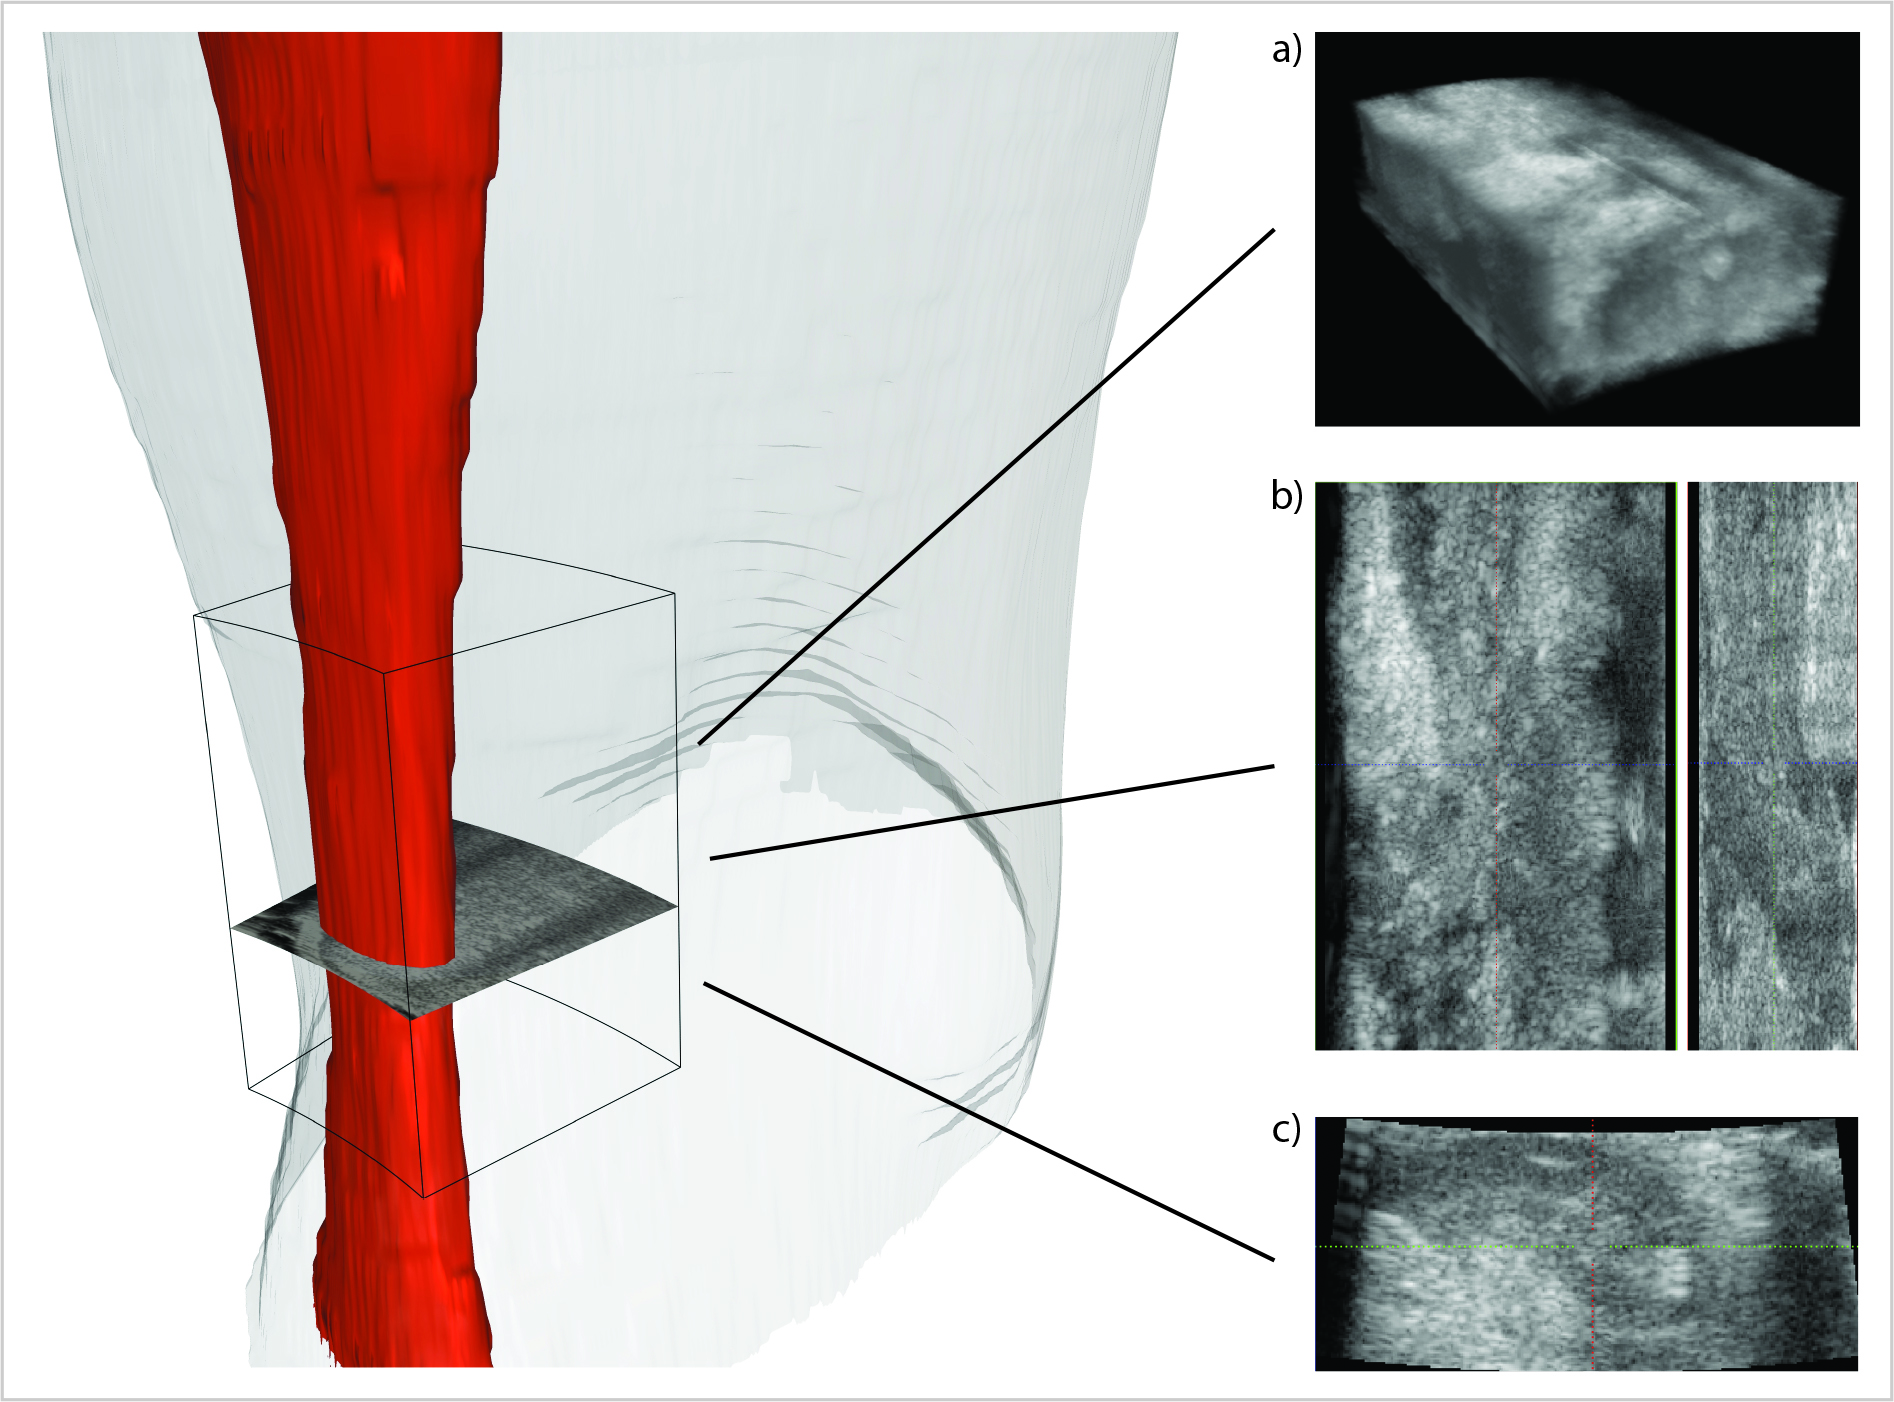
\includegraphics[width=1\textwidth]{figures/sciegnoUSG.jpg}
	\caption{Obszar obrazowania ścięgna Achillesa w USG, wraz z danymi wolumetrycznymi -- a), danymi w przekrojach strzałkowym i czołowym -- b) oraz danymi w przekroju poprzecznym -- c).}
	\label{usgAchillesComp}
\end{figure}


W porównaniu do rezonansu magnetycznego obszar pojedynczego obrazowania jest mniejszy. W kwestii ograniczeń należy również zwrócić uwagę na fakt, że fale akustyczne używane w USG nie propagują się dobrze przez kości i gazy. Zastosowanie do oceny struktur umiejscowionych w otoczeniu lub składających się w większości z takich ośrodków (jak np. mózg lub płuca) znajduje zatem RM. Rezonans Magnetyczny umożliwia również uzyskanie obrazów o lepszej jakości detali. Sam czas badania jest natomiast dłuższy i w większości przypadków niemożliwe jest obrazowanie w czasie rzeczywistym, co z kolei jest naturalne dla techniki USG.

W wymiarze finansowym istotny jest fakt, że aparat do USG kosztuje średnio 10 razy mniej niż aparatura RM. Jak jednak wspomniano, z uwagi na jakość detali, uzyskiwane obrazy są trudniejsze do interpretacji, stąd trudności w  wyszkoleniu kadry. 

Nowe rozwiązania mogą wpłynąć na znaczące zmiany w USG zarówno w warstwie sprzętowej jak i oprogramowania. Po pierwsze postępuje zmiana technologiczna, a przetworniki z piezoelektrykami zastępowane są przetwornikami budowanymi \linebreak w technologi MEMS np. cMUT, czy pMUT (zob. \cite{Butterfly2018})  pozwalające m.in. przetwarzać surowy sygnał ultradźwiękowy (zob. \cite{US4US}). Wynika to z faktu, że dzięki przetwornikom MEMS można wytworzyć cały układ generujący drgania w krzemie w jednym procesie technologicznym razem z dedykowanym układem do zadanej aplikacji (ang. \textit{Application-Specific Integrated Circuit} w skr. \textit{ASIC})\index{ASIC -- skrót od ang. \textit{Application-Specific Integrated Circuit}}. Takie podejście znacząco redukuje koszty oraz implikuje możliwość miniaturyzacji urządzeń.

W warstwie oprogramowania do USG należy zwrócić uwagę na rozwój algorytmów sztucznej inteligencji pozwalających wydobyć i zinterpretować interesującą informację z niskiej jakości obrazów. Przykładowo w \cite{Cunningham2017} algorytmy sztucznej inteligencji zostały użyte do określenia orientacji włókien mięśniowych, a w \cite{NVIDIA-CLARA} \linebreak do segmentacji komór serca w czasie rzeczywistym. 

Obiecujący jest też rozwój metod \textit{UTC}\index{UTC -- skrót od ang. \textit{Ultrasonography Tissue Characterization}} (od ang. Ultrasonography Tissue Characterization). W 2003 r., w \cite{Bakker2003} Bakker et. al. przedstawili pracę pokazującą w jakim stopniu obraz USG jest mieszanką echa związanego z budową tkanki, a w jakim z \textit{interferencji}, czyli nakładania się fal. W zależności od stabilności echa można zatem wnioskować czy obserwowana struktura składa się głównie z dużych, stałych struktur wywołujących stabilne echo, czy np. płynów lub małych włókienek powodujących zmienne interferencje. Jako referencji dla studiowanego echa używa się badań histologicznych (zob. \cite{Bakker2000}). Na tej podstawie sklasyfikowano 4 różne rodzaje echa i jak zasygnalizowano w pracach \cite{vanSchie2009} i \cite{Heyward2018} informacja o proporcjach występowania tych rodzai echa może być użyta do oceny struktury ścięgna Achillesa. Metoda ta nie została jednak jeszcze w pełni zwalidowana i możliwości wnioskowania na jej podstawie \linebreak są wciąż niejasne (zob. \cite{Heyward2018}).

USG i inne techniki obrazowania medycznego nie są jedynymi metodami oceny gojenia się ścięgna Achillesa. W kolejnej sekcji zostały opisane techniki oceny funkcji ścięgna, które samodzielnie jak i w połączeniu z analizą obrazową stanowią wartościową informację diagnostyczną.

\section{Wykorzystanie badań biomechanicznych}
\label{biomechanika}
W poprzednich sekcjach zostały opisane dwie najczęściej wykorzystywane obrazowe metody monitorowania procesu gojenia się ścięgna Achillesa. Komplementarnie, podczas rehabilitacji może być również wykonana \textit{ocena funkcjonalna}, technika weryfikująca w jakim stopniu dany element (tkanka, narząd, organizm) może realizować swoje zadania. W przypadku monitorowania gojenia się ścięgna Achillesa najczęściej w tym celu stosuje się \textit{ocenę biomechaniki}, czyli badania pozwalające wnioskować na temat właściwości mechanicznych elementów składowych organizmów żywych. 

Najbardziej zaawansowane i dokładne metody oceny biomechaniki stosowane współcześnie możliwe są do wykonania przy użyciu urządzeń pomiarowych takich jak:
\begin{itemize}[noitemsep,nolistsep]
	\item \textit{Komputerowa analiza ruchu} (ang. \textit{Motion Capture}) -- narzędzie wykorzystujące systemy czujników do zapisu informacji o zmianach położenia obiektu rejestrowanego np. pacjenta. Do wiodących rozwiązań należy zaliczyć systemy firm Vicon \cite{Vicon}, czy BTS \cite{BTS}.
	\item \textit{Płyty dynamometryczne} (ang. \textit{Force Plates}) -- narzędzie wykorzystywane \linebreak do pomiaru sił reakcji podłoża w trzech prostopadłych płaszczyznach. Dzięki temu można określić sumaryczny udział mięśni w generowaniu sił odpowiadających za balans ciała, ruch w danym kierunku oraz przeciwstawianie się sile grawitacji. Do wiodących rozwiązań należą płyty firmy Kistler \cite{KISTLER}.
	\item \textit{Elektromiografia}, w skr. \textit{EMG}\index{EMG -- elektromiografia} (ang. \textit{Electromyography}) -- narzędzie do pomiaru pobudzeń poszczególnych grup mięśniowych podczas ruchu. Wykorzystywane jest m.in. do określenia rozkładu sił zmierzonych przez płyty dynamometryczne na poszczególne mięśnie.
\end{itemize}

Synchronizacja danych z powyższych urządzeń umożliwia konstrukcję modeli układu mięśniowo-szkieletowego i symulacje funkcji poszczególnych grup mięśniowych oraz ścięgien w zadanych problemach.

Danymi stosowanymi do uszczegółowienia takich modeli są np.: wymiary poszczególnych segmentów ciała (goleń, udo, tors) tzw. pomiary antropometryczne; maksymalne siły izometryczne mierzone z użyciem systemów takich jak Biodex; geometria kości mierzonych np. z pomocą tomografii komputerowej ew. RM; lokalizacja przyczepów mięśniowych określanych przy pomocy RM lub USG; środki masy poszczególnych segmentów określanych np. przy użyciu badania \textit{DXA}\index{DXA -- skrót od ang. \textit{Double X-Ray Absorption}} (od ang. \textit{Double X-Ray Absorption}) lub tomografii komputerowej; charakterystykę włókien mięśniowych widocznych w USG.

Z uwagi na dużą liczbę możliwych do zmierzenia parametrów, ich integracja odbywa się w modelach komputerowych zaimplementowanych w różnego rodzaju oprogramowaniu do symulacji biomechanicznych. Do najczęściej używanych modeli należą opisane w \cite{John2013} Gait 2392 i 2354 oraz obecnie najbardziej złożony -- \textit{AnyBody Full Body Model} \cite{Bassani2017}. 

Historia komputerowo wspomaganego, kompleksowego modelowania biomechaniki ruchu sięga wczesnych lat 90-tych ubiegłego wieku, kiedy to Delp i Loan przedstawili oprogramowanie SIMM \cite{Delp1990}. Obecnie SIMM jak również inne oprogramowania komercyjne takie jak: Visual 3D (Cmotion Inc.) \cite{Visual3D}, Anybody (Anybody Technology) \cite{AnyBody}, czy Adams (MSC Software Corp.) \cite{Adams}, dostarczają narzędzi \linebreak do wartościowych symulacji np. chodu \cite{Steele2010}, biegu \cite{Hamner2010} jak również konsekwencji różnych zabiegów chirurgicznych \cite{Gomes2013} i chorób \cite{Shao2009}. Istnieją również narzędzia otwarte, do których należą szeroko wykorzystywany OpenSim \cite{Delp2007} rozwijany na Uniwersytecie Stanforda, czy też Human Motion \cite{Riken} wywodzący się z instytutu badawczego RIKEN w Japonii.

Powyżej przedstawione kompleksowe badania w praktyce realizowane są rzadko z uwagi na ich wysokie koszty. Dla przykładu w Polsce, ośrodki wyposażone \linebreak w sprzęt pomiarowy takiej klasy to np. Instytut "Pomnik – Centrum Zdrowia Dziecka", Warszawski Uniwersytet Medyczny, Akademia Wychowania Fizycznego imienia Józefa Piłsudskiego, czy komercyjna placówka Fizjofit w Gliwicach. W celu obniżenia kosztów badania stosuje się wybiórcze podejście i selekcję parametrów pomiarowych uznanych przez ekspertów dziedzinowych za wystarczające do analizy zadanego problemu. Dla przykładu, badania stosowane do oceny biomechaniki ścięgna Achillesa w placówce Carolina Medical Center (gdzie zrealizowane były badania wykorzystywane w tej pracy) składają się z następujących pomiarów (zob. \cite{CMC}):

\begin{enumerate}[noitemsep,nolistsep]
	\item Pomiar \textit{ATRS}\index{ATRS -- skrót od ang. \textit{Achilles Tendon Total Rupture Score}} (od ang. \textit{Achilles Tendon Total Rupture Score}) -- oceniany \linebreak w skali od 0 do 100 \cite{NilssonHelander2007} poziom ograniczenia, z którymi pacjenci borykają się w następstwie urazu.
	\item Pomiar stabilograficzny na platformie dynamometrycznej -- mierzone są wychylenia środka ciężkości. Pacjent ma za zadanie utrzymanie równowagi \linebreak na niestabilnym podłożu. Wykonane są dwie próby po 30 sekund kolejno na prawej i lewej kończynie dolnej na dynamicznej platformie dynamometrycznej Biodex Balance System. Wyniki obu prób są porównane między sobą. 
	\item Pomiar stabilograficzny na platformie statycznej -- mierzona jest droga wychylenia środka masy pacjenta w trakcie stania jednonóż na platformie dynamometrycznej, statycznej.
	\item Pomiar sił reakcji na ścieżce podometrycznej -- mierzony jest rozkład sił nacisków podeszwowej strony stóp na podłoże (jedynie w kierunku prostopadłym do podłoża). Pomiar wykonywany jest podczas stania swobodnego, wspięć \linebreak na palce oraz przysiadu bez odrywania pięt. Dokonywana jest również analiza chodu (3 przejścia) i biegu (5 przebiegnięć). Na podstawie sił reakcji wyliczane są parametry: rotacja podudzia [$^\circ$], długość kroków [cm], udział fazy podparcia [\%], udział fazy przenoszenia [\%], maksymalna siła na pięcie [N] oraz maksymalna siła na palcach [N].
	\item Pomiar skoczności i mocy (tzw. siły dynamicznej) kończyn dolnych -- mierzona jest moc maksymalna $P_{max}$\index{$P_{max}$ -- moc maksymalna} i średnia $P_m$\index{$P_m$ -- moc średnia}, maksymalna wysokość uniesienia $h_{max}$\index{$h_{max}$ -- maksymalna wysokość uniesienia środka masy ciała przed odbiciem} i obniżenia $h_{min}$\index{$h_{min}$ -- minimalna wysokość uniesienia środka masy ciała przed odbiciem} środka masy ciała przed odbiciem. Wykonywane są wyskoki pionowe z miejsca na platformie dynamometrycznej. Realizowane są dwie próby obunóż oraz na prawej i lewej kończynie dolnej. W celu pełnego zaangażowania kończyn dolnych pacjent podczas badania trzyma ręce na biodrach. 
	\item Pomiary momentów sił mięśni stawu skokowego -- mierzone są maksymalne wartości momentu siły mięśni zginaczy podeszwowych i grzbietowych stawu skokowego [Nm] oraz deficyt pomiędzy operowaną i zdrową kończyną dolną [\%]. Momenty sił mierzone są w dwóch pozycjach tj. z wyprostowanym oraz zgiętym do 50 stopni stawem kolanowym \cite{Orishimo2008}. Pomiar realizowany jest w warunkach izometrii i izokinetyki w trzech prędkościach kątowych 60$^\circ$/s (5 powtórzeń), 120$^\circ$/s (8 powtórzeń) oraz 180$^\circ$/s (10 powtórzeń) przy wykorzystaniu urządzenia Humac Norm (USA). Przed badaniem pacjent odbywa 5 minutową rozgrzewkę na steperze.
\end{enumerate}

Wymienione badania zostały określone przez ortopedów i fizjoterapeutów jako wystarczające do oceny przywracania funkcji ścięgna Achillesa po rekonstrukcji. 

Wraz z oceną strukturalną realizowaną poprzez badania obrazowe i wiedzą ekspercką, informacja tak zgromadzona może służyć do subiektywnego monitorowania procesu gojenia się ścięgna. Do skutecznej obiektywizacji tego procesu potrzebne są jednak dodatkowe metody bazujące na agregacji ilościowych współczynników \linebreak i automatycznym wnioskowaniu na ich podstawie. Do tej grupy należą algorytmy sztucznej inteligencji opisane dalej w pracy. 